\PassOptionsToPackage{english}{babel}
\documentclass{report}
\usepackage[utf8]{inputenc}

%\usepackage[english]{babel}
%\usepackage[latin1]{inputenc}
%\usepackage{geometry}
%\usepackage{listings}
\usepackage{caption}
\usepackage{amsmath}
\usepackage{graphics}
\usepackage[T1]{fontenc}
\usepackage{enumitem} %bold enumeration
\usepackage[utf8]{inputenc}
\usepackage[english]{babel}
%\usepackage{pmgraph}
\usepackage{mathrsfs}
\usepackage{floatflt}
\usepackage{multicol}
\usepackage{color,colortbl}
% \usepackage[pdftex]{graphicx}
\usepackage[normalem]{ulem}
\usepackage[colorlinks,urlcolor=blue, linkcolor=blue]{hyperref}
\usepackage{epstopdf}
\usepackage{wrapfig}
\usepackage{multirow}
%% Sets page size and margins
\usepackage[a4paper,top=3cm,bottom=2cm,left=3cm,right=3cm,marginparwidth=1.75cm]{geometry}
%% Useful packages
\usepackage[colorinlistoftodos]{todonotes}
\usepackage{xymtex}
\usepackage{fancyhdr}
\usepackage{epstopdf}
\usepackage{indentfirst} \geometry{verbose,a4paper,tmargin=3cm,bmargin=3cm,lmargin=1.0cm,rmargin=2.0cm}
\setlength{\parindent}{0pt}
 \graphicspath{C:/Users/Anton/Desktop/ETH_books/CV/CV-Lab-Model-Fitting/CV-Lab-Model-Fitting/src/epipolar_geometry/res}
\begin{document}
\large
Report of Anton Maksimov (antonma, 16-952-137), Task 6 "Model fitting"\\
 on ETHZ course "Computer Vision".\\
\rule{\linewidth}{1pt}
%%%%%%%%%%%%%%%%%%%%%%%%%%%%%%%%%%%%%%%%%%%%%%%%%%%%%%%%%   1
	\textbf{1.} We implement more efficient for MATLAB matrix version of SSD map calculation, smooth it using averaging filters --- boxes of different sizes. Using this map we find the best dispairity for each pixel and save it. 
	
	We can see that the more is size of the filter, the more smooth is the picture and more connected areas are present.
	\begin{figure}[h]
		\begin{center}
			\begin{minipage}[h]{0.45\linewidth}
				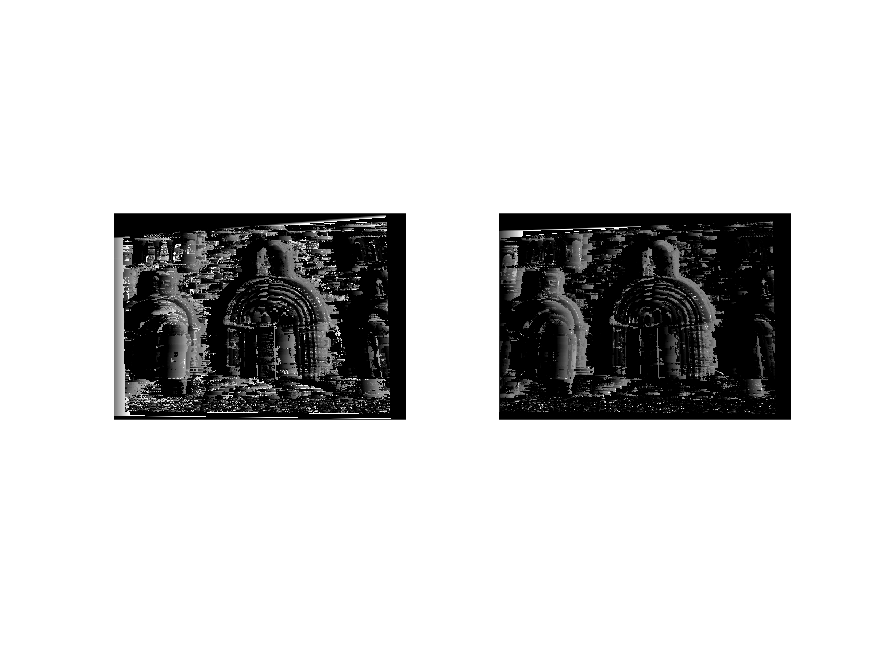
\includegraphics[width=1\linewidth, trim = {2cm 3.5cm 8cm 3.5cm}, clip]{C:/Users/Anton/Desktop/ETH_books/CV/cv_lab06_stereo_matching_2019/cv_lab06_stereo_matching/code/results/SD_3}
				\caption{3x3}
			\end{minipage}
		\hfill
		\begin{minipage}[h]{0.45\linewidth}
			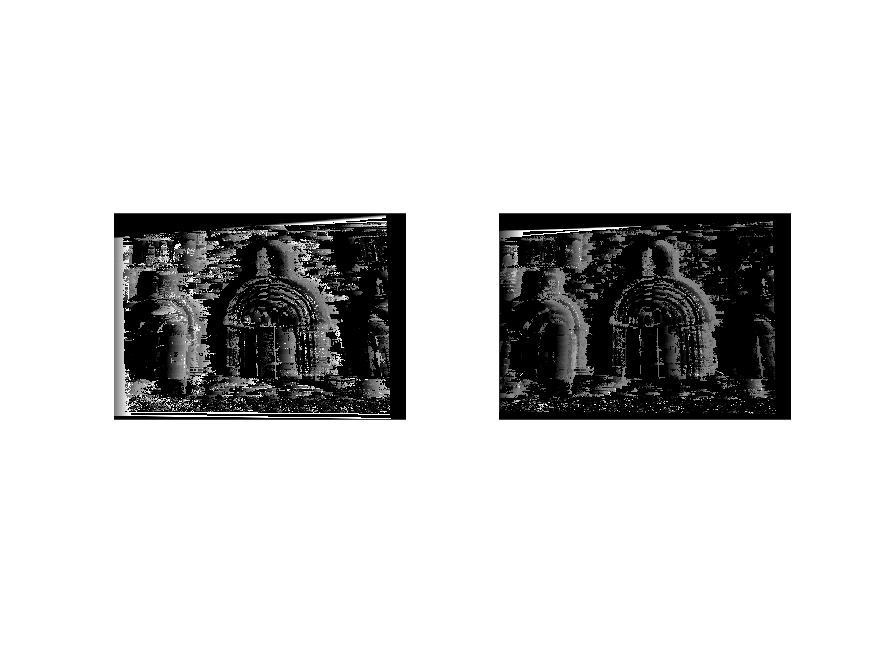
\includegraphics[width=1\linewidth, trim = {2cm 3.5cm 8cm 3.5cm}, clip]{C:/Users/Anton/Desktop/ETH_books/CV/cv_lab06_stereo_matching_2019/cv_lab06_stereo_matching/code/results/SD_7}
			\caption{7x7}
		\end{minipage}
	\vfill
	\begin{minipage}[h]{0.45\linewidth}
		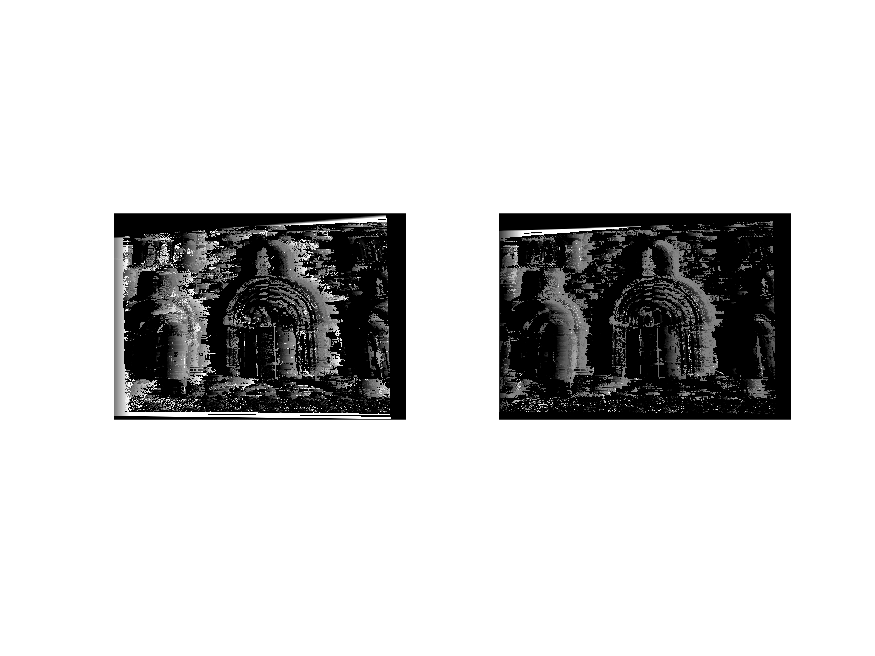
\includegraphics[width=1\linewidth, trim = {2cm 3.5cm 8cm 3.5cm}, clip]{C:/Users/Anton/Desktop/ETH_books/CV/cv_lab06_stereo_matching_2019/cv_lab06_stereo_matching/code/results/SD_12}
		\caption{12x12}
	\end{minipage}
		\end{center}
	\caption{Dispairity maps for <<winner--takes--all>> and different sizes of box filter.}
	\end{figure}

	\begin{figure}[h]
	\begin{center}
		\begin{minipage}[h]{0.3\linewidth}
			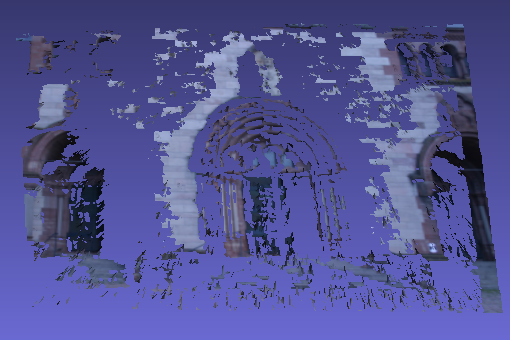
\includegraphics[width=1\linewidth]{C:/Users/Anton/Desktop/ETH_books/CV/cv_lab06_stereo_matching_2019/cv_lab06_stereo_matching/results/SD_3x3_rng40_3d}
			\caption{3x3}
		\end{minipage}
		\hfill
		\begin{minipage}[h]{0.3\linewidth}
			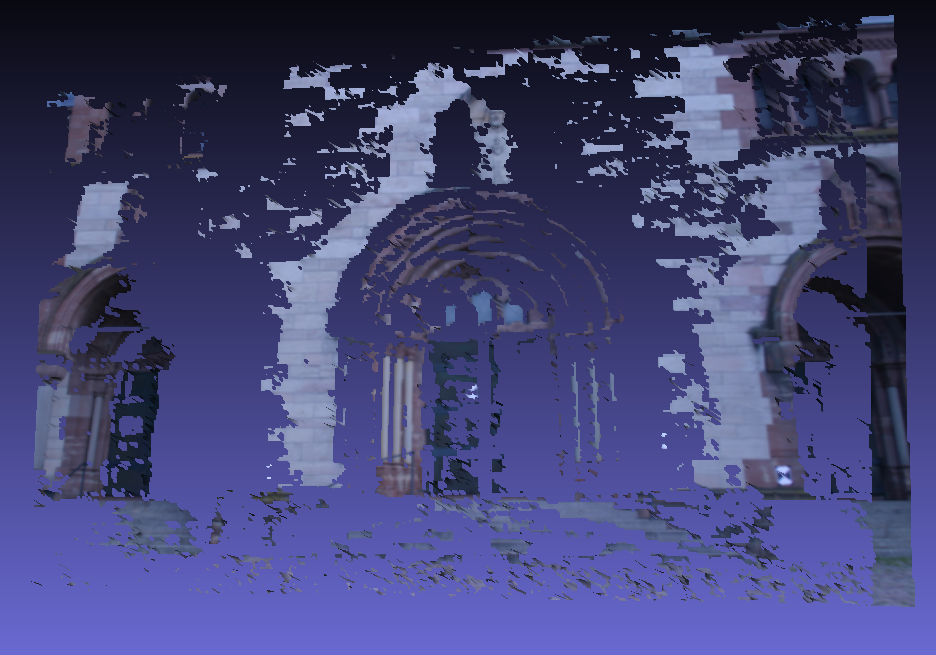
\includegraphics[width=1\linewidth]{C:/Users/Anton/Desktop/ETH_books/CV/cv_lab06_stereo_matching_2019/cv_lab06_stereo_matching/results/SD_10x10_rng40_3d}
			\caption{10x10}
		\end{minipage}
		\hfill
		\begin{minipage}[h]{0.3\linewidth}
			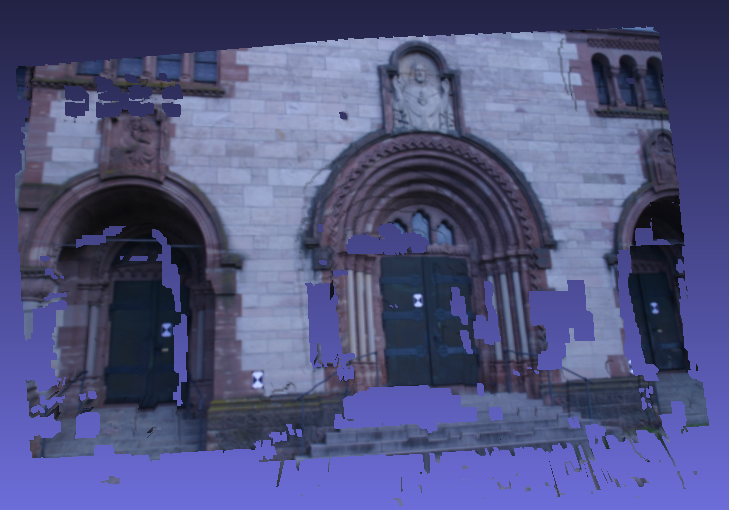
\includegraphics[width=1\linewidth]{C:/Users/Anton/Desktop/ETH_books/CV/cv_lab06_stereo_matching_2019/cv_lab06_stereo_matching/results/SD_20x20_rng40_3d}
			\caption{20x20}
		\end{minipage}
	\end{center}
	\caption{3D-reconstructions for <<winner--takes--all>> and different sizes of box filter..}
\end{figure}

\newpage
%%%%%%%%%%%%%%%%%%%%%%%%%%%%%%%%%%%%%%%%%%%%%%%%%%%%%%%%%   2
\section{2}
	\textbf{2.} We apply graph-cut algorithm for classification of pixels (labeling them with the best value of dispairity), where cost of labeling consists of price to label pixel, which is taken from correspondent SSD, and price of changing label relatively to neighboring pixels, which comes from gaussian filtering (i.e. considers local gradient of intensity). Graph-cut algorithm gives much better results than the previous algorithm, labeling is smoother and uniformer, it has problems only in places of fast change of deepness.
	
	Size of averaging filter is connected with parameters of GraphCut (there are parameters which control smoothness), so we just use 3x3 filter here. In order to search for the best parameters, we change coefficients DataCost (second parameter) and SmoothnessCost (third parameter) of function Graph, choose the best. As the further improvement wee could after that change size and covariance of gaussian filter and choose the best from them.
	
	The best looks with DataCost 100 and SmoothnessCost 2 coefficients.
	\begin{figure}[h]
		\begin{center}
			\begin{minipage}[h]{0.49\linewidth}
				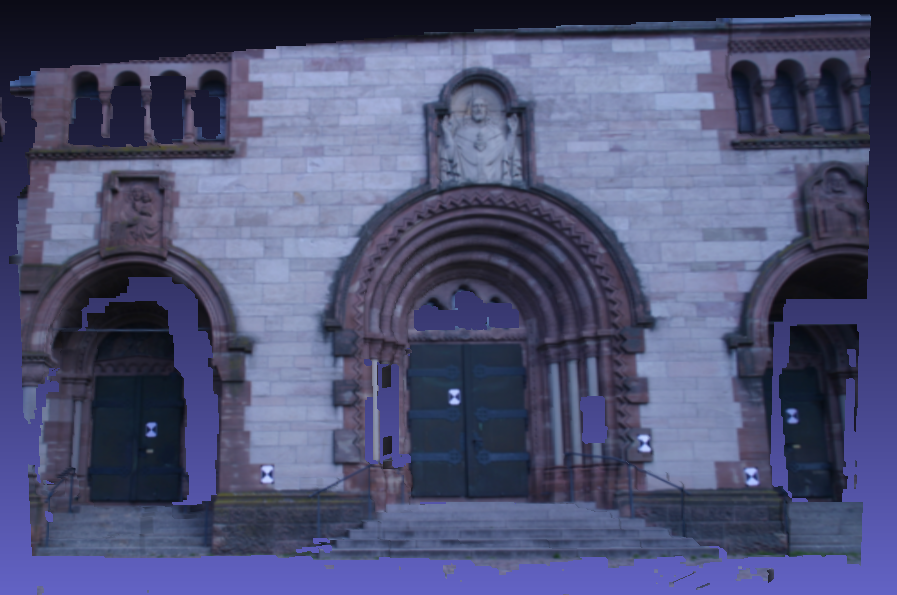
\includegraphics[width=1\linewidth]{C:/Users/Anton/Desktop/ETH_books/CV/cv_lab06_stereo_matching_2019/cv_lab06_stereo_matching/results/SG_3_1000_5_5_5}
			\end{minipage}
		\caption{GraphCut. One of the results with coeff near DataCost 1000, near SmoothnessCost 5, gaussian filter size 3 and covariance 3.}
		\end{center}
	\end{figure}

\begin{figure}[h]
	\begin{center}
		\begin{minipage}[h]{0.45\linewidth}
			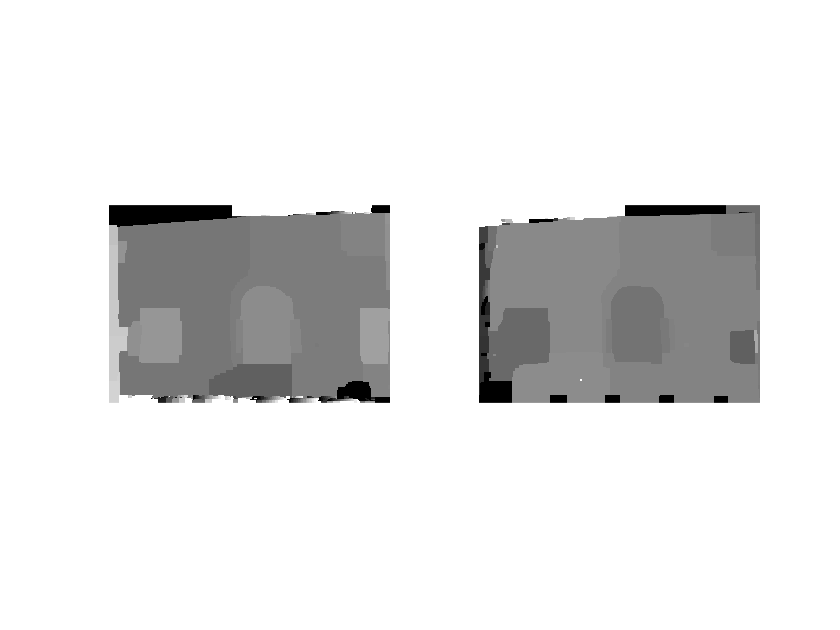
\includegraphics[width=1\linewidth, trim = {2cm 4cm 11cm 4cm}, clip]{C:/Users/Anton/Desktop/ETH_books/CV/cv_lab06_stereo_matching_2019/cv_lab06_stereo_matching/code/results/GC_3_100_2_5_5_map}
		\end{minipage}
		\hfill
		\begin{minipage}[h]{0.45\linewidth}
			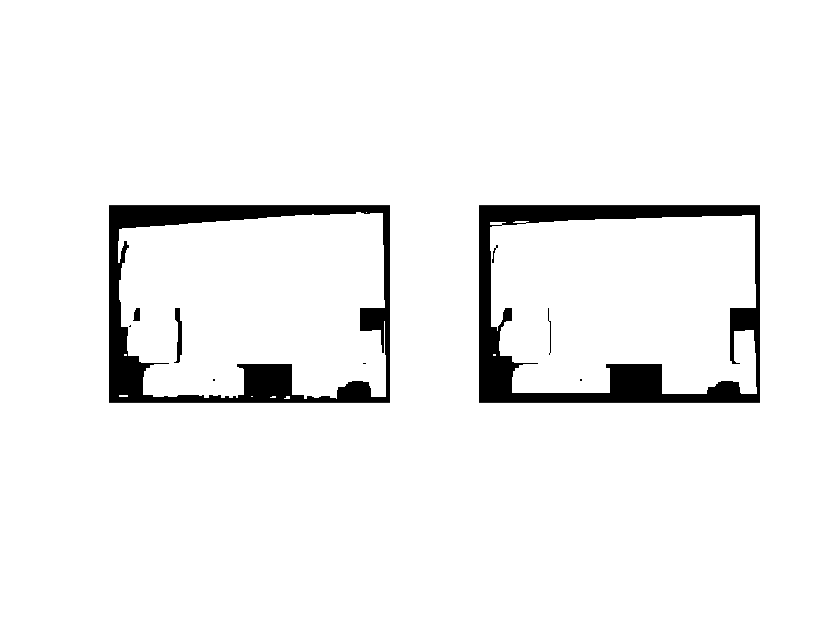
\includegraphics[width=1\linewidth, trim = {2cm 4cm 11cm 4cm}, clip]{C:/Users/Anton/Desktop/ETH_books/CV/cv_lab06_stereo_matching_2019/cv_lab06_stereo_matching/code/results/GC_3_100_2_5_5_mask}			
		\end{minipage}
		\caption{GraphCut. DataCost 100, SmoothnessCost 2, Gaussian size 3, covariance 3}
	\end{center}
\end{figure}
\begin{figure}[h]
	\begin{center}
		\begin{minipage}[h]{0.45\linewidth}
			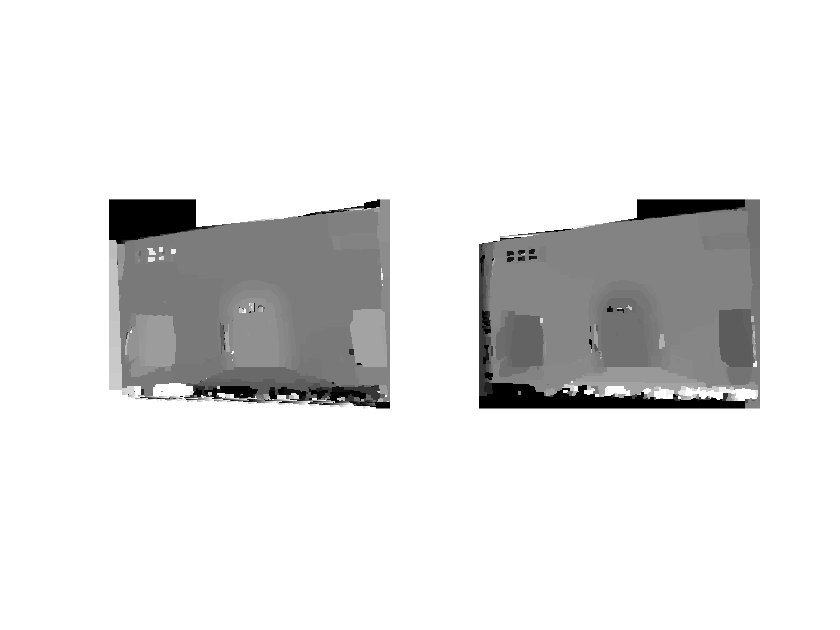
\includegraphics[width=1\linewidth, trim = {2cm 4cm 11cm 4cm}, clip]{C:/Users/Anton/Desktop/ETH_books/CV/cv_lab06_stereo_matching_2019/cv_lab06_stereo_matching/code/results/GC_3_500_2_5_5_map}
		\end{minipage}
		\hfill
		\begin{minipage}[h]{0.45\linewidth}
			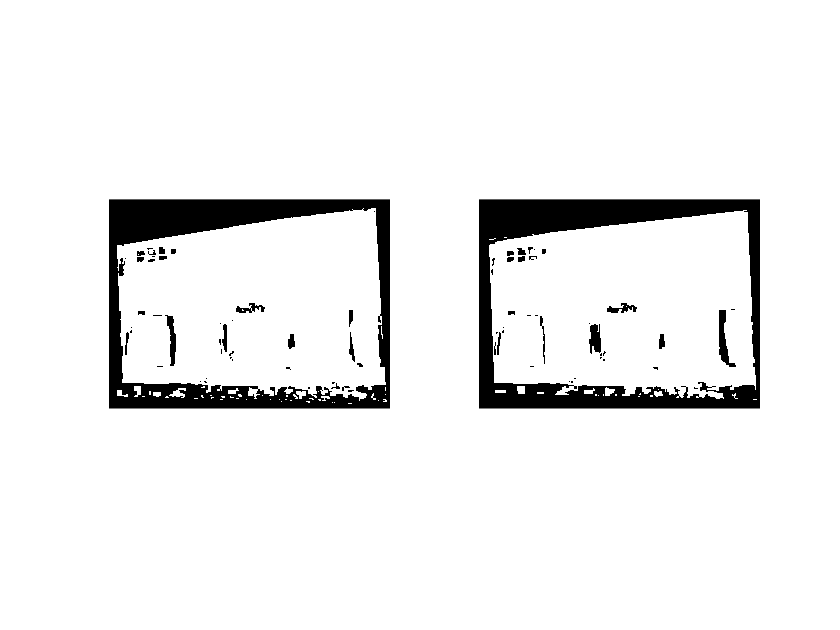
\includegraphics[width=1\linewidth, trim = {2cm 4cm 11cm 4cm}, clip]{C:/Users/Anton/Desktop/ETH_books/CV/cv_lab06_stereo_matching_2019/cv_lab06_stereo_matching/code/results/GC_3_500_2_5_5_mask}			
		\end{minipage}
	\caption{GraphCut. DataCost 500, SmoothnessCost 2, Gaussian size 3, covariance 3}
	\end{center}
\end{figure}
\begin{figure}[h]
	\begin{center}
		\begin{minipage}[h]{0.45\linewidth}
			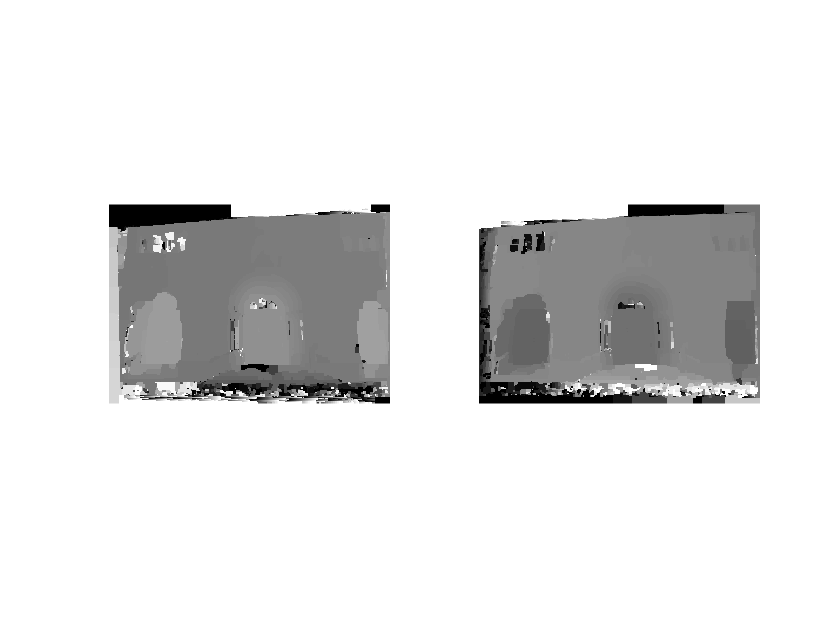
\includegraphics[width=1\linewidth, trim = {2cm 4cm 11cm 4cm}, clip]{C:/Users/Anton/Desktop/ETH_books/CV/cv_lab06_stereo_matching_2019/cv_lab06_stereo_matching/code/results/GC_3_1000_2_5_5_map}
		\end{minipage}
		\hfill
		\begin{minipage}[h]{0.45\linewidth}
			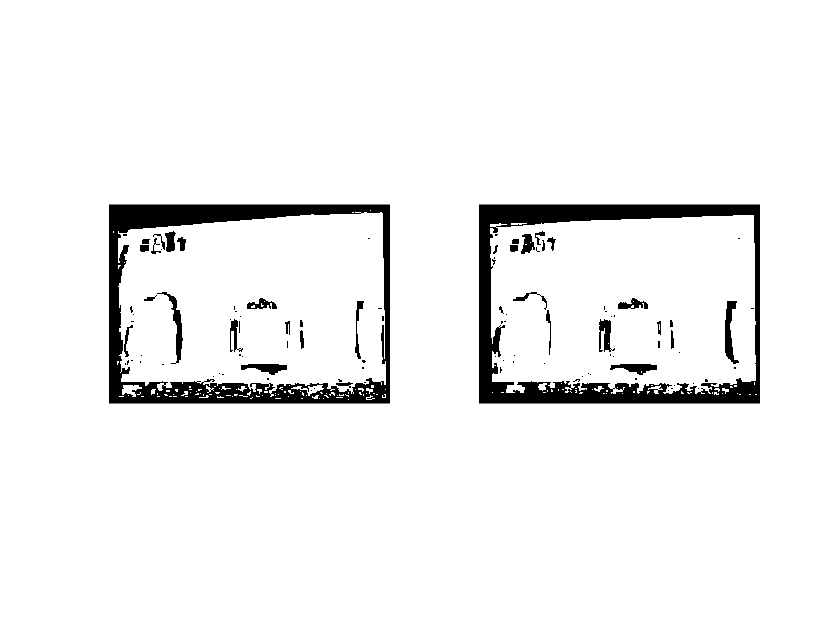
\includegraphics[width=1\linewidth, trim = {2cm 4cm 11cm 4cm}, clip]{C:/Users/Anton/Desktop/ETH_books/CV/cv_lab06_stereo_matching_2019/cv_lab06_stereo_matching/code/results/GC_3_1000_2_5_5_mask}			
		\end{minipage}
		\caption{GraphCut. DataCost 1000, SmoothnessCost 2, Gaussian size 3, covariance 3}
	\end{center}
\end{figure}
\begin{figure}[h]
	\begin{center}
		\begin{minipage}[h]{0.45\linewidth}
			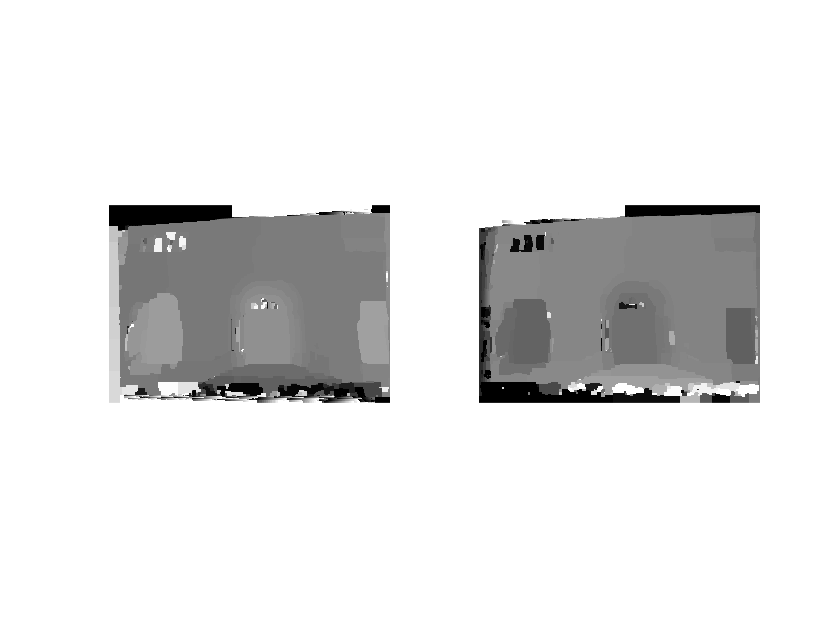
\includegraphics[width=1\linewidth, trim = {2cm 4cm 11cm 4cm}, clip]{C:/Users/Anton/Desktop/ETH_books/CV/cv_lab06_stereo_matching_2019/cv_lab06_stereo_matching/code/results/GC_3_1000_5_5_5_map}
		\end{minipage}
		\hfill
		\begin{minipage}[h]{0.45\linewidth}
			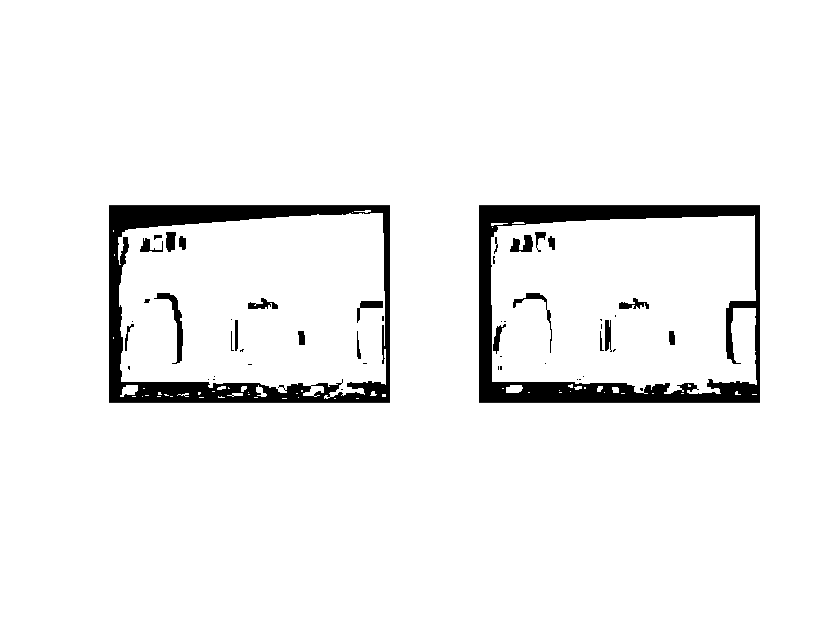
\includegraphics[width=1\linewidth, trim = {2cm 4cm 11cm 4cm}, clip]{C:/Users/Anton/Desktop/ETH_books/CV/cv_lab06_stereo_matching_2019/cv_lab06_stereo_matching/code/results/GC_3_1000_5_5_5_mask}			
		\end{minipage}
		\caption{GraphCut. DataCost 1000, SmoothnessCost 5, Gaussian size 3, covariance 3}
	\end{center}
\end{figure}

The best looks with 100 and 2 coefficients.
\begin{figure}[h]
	\begin{center}
		\begin{minipage}[h]{0.49\linewidth}
			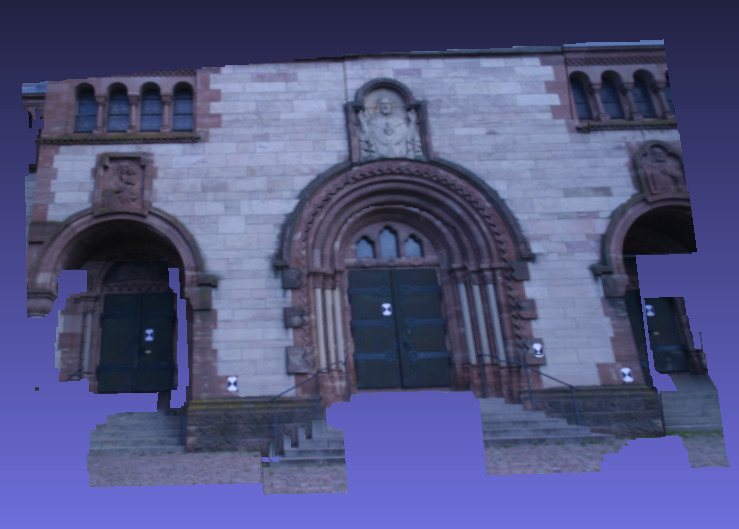
\includegraphics[width=1\linewidth]{C:/Users/Anton/Desktop/ETH_books/CV/cv_lab06_stereo_matching_2019/cv_lab06_stereo_matching/results/SG_3_100_2_5_5}
		\end{minipage}
		\hfill
		\begin{minipage}[h]{0.49\linewidth}
			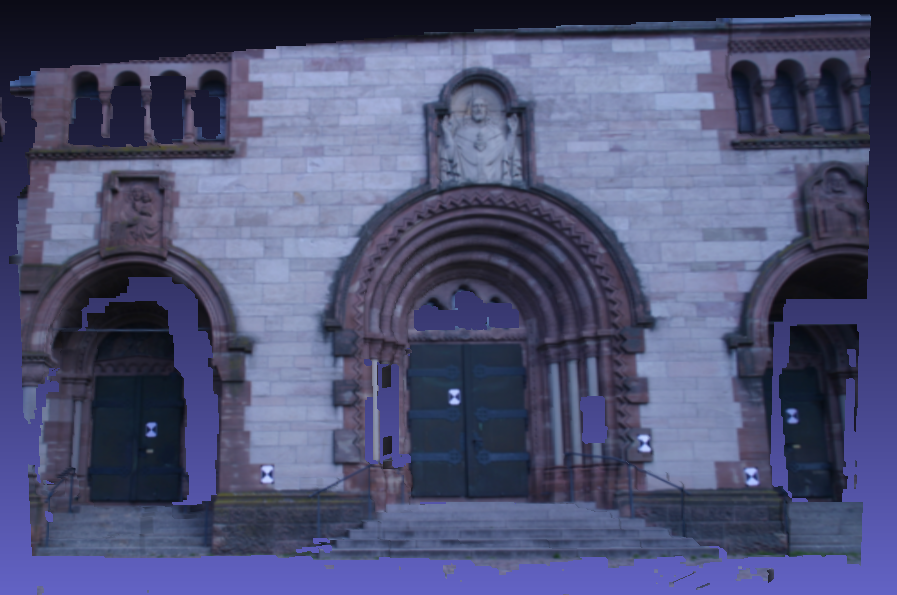
\includegraphics[width=1\linewidth]{C:/Users/Anton/Desktop/ETH_books/CV/cv_lab06_stereo_matching_2019/cv_lab06_stereo_matching/results/SG_3_1000_5_5_5}
		\end{minipage}
		\caption{GraphCut. The best found combination of parameters improves quality (left --- DataCost 100 and SmoothnessCost 2, right -- 1000 and 5).}
	\end{center}
\end{figure}
%%%%%%%%%%%%%%%%%%%%%%%%%%%%%%%%%%%%%%%%%%%%%%%%%%%%%%%%%   3
\newpage
\textbf{3.} In order to estimate range of disparities of the image we get disparities of points of interest from RANSAC on extracted by SIFT
matches. We approximate range of disparities as maximal shift among this
matching points along horizontal axis multiplied by 2 in order to make
it more robust against existence of areas with no points of interest but
bigger dispairity value.

In order to get enough matches we start from small threshold for Sampson distance of inliers in RANSAC and multiply it by 10 every step while we don't get 50 matches. So, this number of inliers is essentially the only parameter needed to be chosen in order to get range of dispairities.

We used function \texttt{fundamentalMatrixRANSAC}, but introduced \texttt{threshold} as a parameter, so we can iteratively change accuracy of search.

For given images we estimated maximal dispairity (multiplied by 2) as 25--30 during several launches. It workes faster as needs less iterations over dispairity range, quality is the same more or less.

\begin{figure}[h]
	\begin{center}
		\begin{minipage}[h]{0.95\linewidth}
			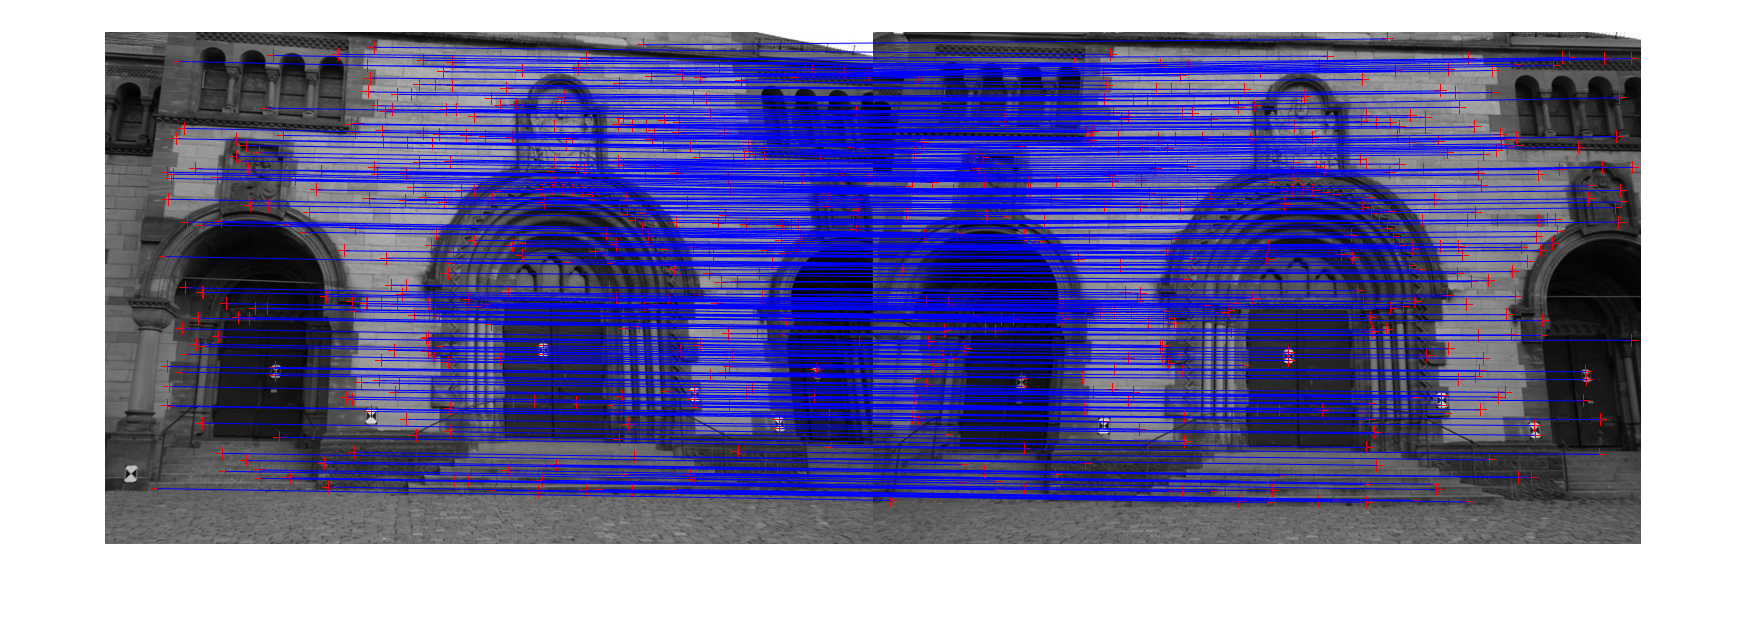
\includegraphics[width=1\linewidth, trim = {0cm 0cm 0cm 0cm}, clip]{C:/Users/Anton/Desktop/ETH_books/CV/cv_lab06_stereo_matching_2019/cv_lab06_stereo_matching/results/ransac}
		\end{minipage}
	\caption{Matches obtained by RANSAC from which we estimate the range of search of dispairities.}
	\end{center}
\end{figure}
\end{document}